\documentclass[tikz,border=10pt]{standalone}
\usepackage{amsmath}
\usetikzlibrary{arrows.meta}
\begin{document}
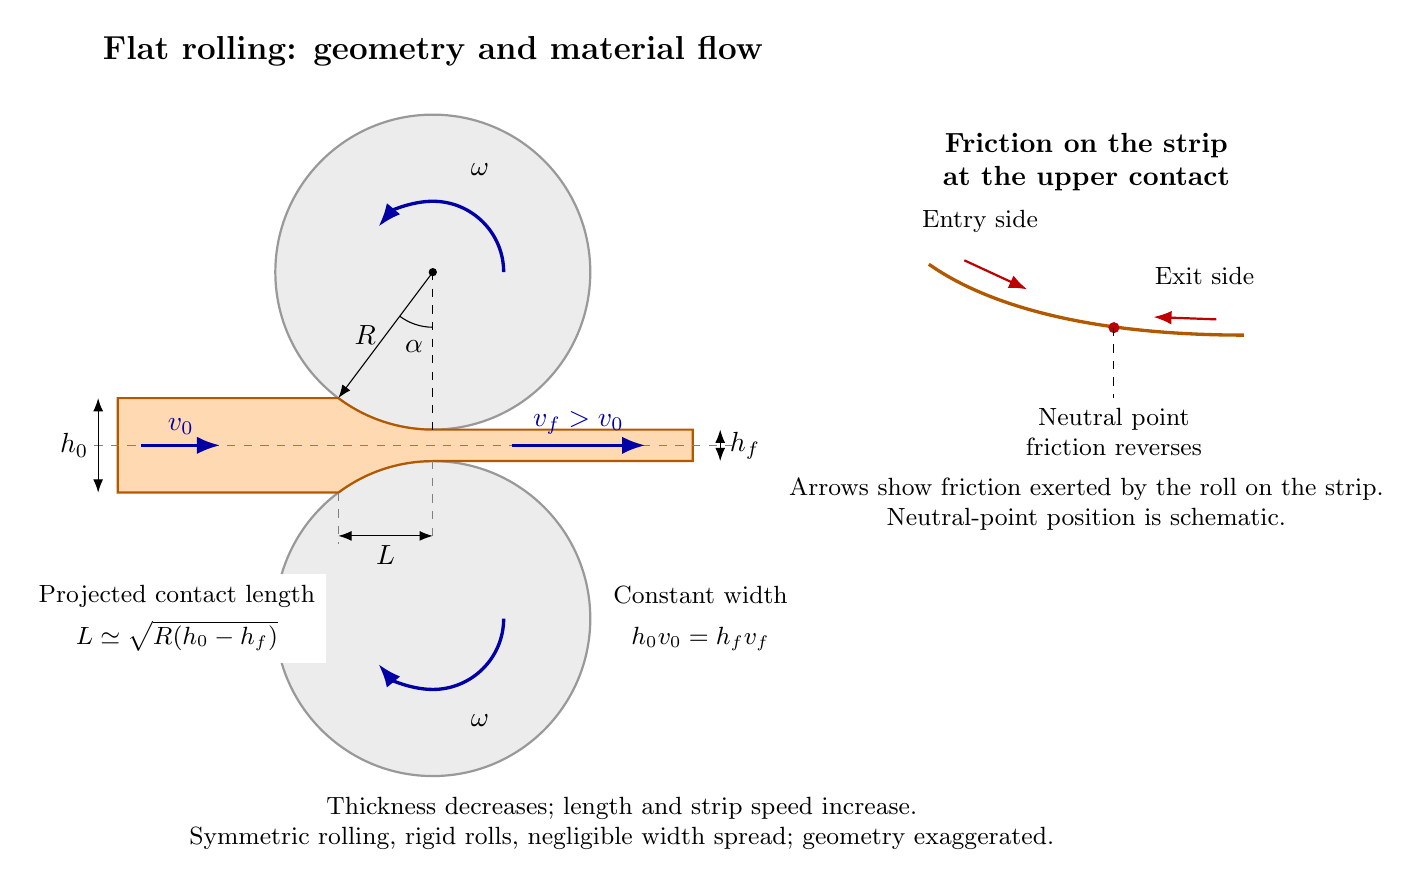
\begin{tikzpicture}[>=Latex,font=\sffamily,
 flow/.style={->,blue!65!black,very thick},
 dim/.style={<->,thin},friction/.style={->,red!75!black,thick}]
\node[font=\bfseries\large] at (0,5) {Flat rolling: geometry and material flow};
% Exact schematic geometry: R=2, hf=0.4, h0=1.2, L=1.2.
\filldraw[fill=gray!15,draw=gray!80,thick] (0,2.2) circle (2);
\filldraw[fill=gray!15,draw=gray!80,thick] (0,-2.2) circle (2);
\path[fill=orange!30,draw=orange!70!black,thick]
 (-4,0.6)--(-1.2,0.6)
 arc[start angle=233.130102,end angle=270,radius=2]
 --(3.3,0.2)--(3.3,-0.2)--(0,-0.2)
 arc[start angle=90,end angle=126.869898,radius=2]
 --(-4,-0.6)--cycle;
\draw[dashed,gray] (-4.3,0)--(3.8,0);
\draw[flow] (-3.7,0)--(-2.7,0) node[midway,above] {$v_0$};
\draw[flow] (1,0)--(2.7,0) node[midway,above] {$v_f>v_0$};
\draw[dim] (-4.25,-0.6)--(-4.25,0.6) node[midway,left] {$h_0$};
\draw[dim] (3.65,-0.2)--(3.65,0.2) node[midway,right] {$h_f$};
\fill (0,2.2) circle (1.5pt);
\draw[->] (0,2.2)--(-1.2,0.6) node[midway,left] {$R$};
\draw[dashed] (0,2.2)--(0,0.2);
\draw (0,1.5) arc[start angle=270,end angle=233.130102,radius=0.7];
\node at (-0.24,1.25) {$\alpha$};
% Top roll CCW and bottom roll CW drive strip to the right.
\draw[flow] (0.9,2.2) arc[start angle=0,end angle=140,radius=0.9];
\node at (0.6,3.5) {$\omega$};
\draw[flow] (0.9,-2.2) arc[start angle=0,end angle=-140,radius=0.9];
\node at (0.6,-3.5) {$\omega$};
\draw[dashed,gray] (-1.2,-0.6)--(-1.2,-1.25);
\draw[dashed,gray] (0,-0.2)--(0,-1.25);
\draw[dim] (-1.2,-1.15)--(0,-1.15) node[midway,below] {$L$};
\node[align=center,font=\small,fill=white,inner sep=4pt] at (-3.25,-2.2)
 {Projected contact length\\[4pt]$L\simeq\sqrt{R(h_0-h_f)}$};
\node[align=center,font=\small] at (3.4,-2.2)
 {Constant width\\[4pt]$h_0v_0=h_fv_f$};

% Separate conceptual contact view avoids clutter in the roll gap.
\begin{scope}[shift={(6.3,1.4)}]
\node[font=\bfseries,align=center] at (2,2.2) {Friction on the strip\\at the upper contact};
\draw[orange!70!black,very thick] (0,0.9)..controls(1,0.2)and(2.6,0)..(4,0);
\draw[friction] (0.45,0.95)--(1.25,0.58);
\draw[friction] (3.65,0.2)--(2.85,0.23);
\fill[red!75!black] (2.35,0.095) circle (2pt);
\draw[dashed] (2.35,0.095)--(2.35,-0.8);
\node[below,align=center,font=\small] at (2.35,-0.8) {Neutral point\\friction reverses};
\node[font=\small] at (0.65,1.45) {Entry side};
\node[font=\small] at (3.5,0.75) {Exit side};
\node[align=center,font=\small] at (2,-2.15)
 {Arrows show friction exerted by the roll on the strip.\\
  Neutral-point position is schematic.};
\end{scope}
\node[font=\small,align=center] at (2.4,-4.8)
 {Thickness decreases; length and strip speed increase.\\
  Symmetric rolling, rigid rolls, negligible width spread; geometry exaggerated.};
\end{tikzpicture}
\end{document}
